\documentclass[pra,12pt]{revtex4}
\usepackage{amsmath}
\usepackage{amssymb}
\usepackage{graphicx}
\usepackage{color}
\usepackage{mathrsfs}
\usepackage[pdfborder={0 0 0},colorlinks=true,linkcolor=blue]{hyperref}

\def\ket#1{\left|#1\right\rangle}
\def\bra#1{\left\langle#1\right|}
\def\braket#1{\left\langle#1\right\rangle}

\setlength{\parindent}{0pt}

\renewcommand{\baselinestretch}{1.0}
\setlength{\parskip}{0.07in}

\begin{document}

\begin{center}
{\Large \textbf{Chapter 2: Quantum Entanglement}}
\end{center}

\section{Quantum mechanics of multi-particle systems}

So far, we have studied quantum mechanical systems consisting of
single particles.  The next important step is to look at systems of
more than one particle.  As we shall see, the postulates of quantum
mechanics have interesting implications that only show up in
multi-particle systems, particularly the phenomenon of \textbf{quantum
  entanglement}.

In the following discussion, you may assume we are dealing with
systems of ``distinguishable'' particles.  There is another set of
complications if the particles are ``identical'' or
``indistinguishable'', which we'll deal with in the next chapter.  (If
you're unsure what this means, just read on.)

Suppose we have a pair of distinguishable particles, labeled A and B.
If each individual particle is treated as a quantum system, then
according to the postulates of quantum mechanics, its state is
described by a vector in a complex Hilbert space.  Let $\mathscr{H}_A$
and $\mathscr{H}_B$ denote the respective single-particle Hilbert
spaces.  When the two particles are considered as a single system, the
combined Hilbert space is denoted
$$\mathscr{H} = \mathscr{H}_A\otimes \mathscr{H}_B.$$
The symbol $\otimes$ refers to a \textbf{tensor product}, which is a
mathematical operation that combines two Hilbert spaces to form
another Hilbert space.  Its meaning is as follows: let $\mathscr{H}_A$
be spanned by an orthonormal basis $\{|\mu_1\rangle, |\mu_2\rangle,
|\mu_3\rangle, \dots\}$, and $\mathscr{H}_B$ spanned by
$\{|\nu_1\rangle, |\nu_2\rangle, |\nu_3\rangle, \dots\}$.  Then
$\mathscr{H}_A \otimes \mathscr{H}_B$ is a space spanned by the basis
vectors
$$\Big\{\;\,|\mu_i\rangle\otimes|\nu_j\rangle \;\;  \Big| \;\; \textrm{all}\;|\mu_i\rangle,\; |\nu_j\rangle \;\,\Big\}.$$
This reflects the intuitive notion that if particle A has some state
$|\mu_i\rangle$ and particle B has state $|\nu_j\rangle$, then the
state of the combined system is fully specified.  Note that if
$\mathscr{H}_A$ has dimension $d_A$ and $\mathscr{H}_B$ has dimension
$d_B$, then the combined Hilbert space $\mathscr{H}$ has dimension
$d_A d_B$.  Using such a basis, any two-particle state can be written as
$$|\psi\rangle = \sum_{i} \sum_{j} \, c_{ij}\; |\mu_i\rangle \otimes |\nu_j\rangle.$$

The inner product between the tensor product basis states is defined
as follows:
$$\Big(|\mu_i\rangle \otimes |\nu_j\rangle\;,\; |\mu_p\rangle \otimes |\nu_q\rangle \Big) \;\equiv\; \Big(\langle\mu_i| \otimes \langle\nu_j| \Big) \Big(|\mu_p\rangle \otimes |\nu_q\rangle\Big) \;\equiv\; \langle\mu_i|\mu_p\rangle \, \langle\nu_j|\nu_q\rangle = \delta_{ip}\delta_{jq}.$$
In other words, we (i) calculate the inner product for space A, (ii)
calculate the inner product for space B, and (iii) multiply the two
resulting numbers together.  You can check that this satisfies the
formal requirements for an inner product in linear algebra.

As an example, suppose $\mathscr{H}_A$ and $\mathscr{H}_B$ are both 2D
Hilbert spaces describing spin-$1/2$ degrees of freedom.  Each space
can be spanned by an orthonormal basis $\{\,|\!+\!z\rangle,
\,|\!-\!z\rangle \, \}$, representing ``spin-up'' and ``spin-down''.
Then the tensor product space $\mathscr{H}$ is a 4D space spanned by
$$\Big\{\;|\!+\!z\rangle\otimes|\!+\!z\rangle\,,\; |\!+\!z\rangle\otimes|\!-\!z\rangle\,,\; |\!-z\!\rangle\otimes|\!+\!z\rangle\,,\; |\!-\!z\rangle\otimes|\!-\!z\rangle \;\Big\}.$$

We now make an important observation.  As previously noted, if
particle $A$ is in state $|\mu_i\rangle$ and particle $B$ is in state
$|\nu_j\rangle$, that specifies the state of the combined system.  But
the reverse is not generally true!  There are states of the combined
system that \textit{cannot} be expressed in terms of definite states
of the individual particles.  For example, take the previous example
of two spaces describing spin-$1/2$ degrees of freedom, and consider
$$|\psi\rangle = \frac{1}{\sqrt{2}} \Big(|\!+\!z\rangle\otimes|\!-\!z\rangle \,-\, |\!-\!z\rangle\otimes|\!+\!z\rangle\Big).$$

This two-particle state is constructed from two of the basis states of
the tensor product space, $|\!+\!z\rangle\otimes|\!-\!z\rangle$ and
$|\!-\!z\rangle\otimes|\!+\!z\rangle$; you can check that the factor
of $1/\sqrt{2}$ normalizes the state so that $\langle\psi|\psi\rangle
= 1$.  Evidently, neither particle A nor particle B has a definite
$|\!+\!z\rangle$ or $|\!-\!z\rangle$ state.  Moreover, we shall show
(in Section~\ref{sec:entropy}) that there's \textit{no} choice of
basis that allows the individual particles to be expressed with
definite quantum states; i.e.,
$$|\psi\rangle \ne |\psi_A\rangle\otimes|\psi_B\rangle \;\;\;\textrm{for}\;\textrm{any}\;\; |\psi_A\rangle \in \mathscr{H}_A, \;|\psi_B\rangle \in \mathscr{H}_B.$$
In such a situation, the two particles are said to be
\textbf{entangled}.  They cannot be described by individual
single-particle quantum states, but are intrinsically ``mixed
together''.

For systems of more than two particles, quantum states can be defined
using multiple tensor products.  In general, suppose a quantum system
contains $N$ subsystems described by the individual Hilbert spaces
$\{\mathscr{H}_1, \mathscr{H}_2, \dots, \mathscr{H}_N\}$, which have
dimensionality $\{d_1, \dots, d_N\}$.  Then the overall system is
described by the Hilbert space
$$\mathscr{H} = \mathscr{H}_1 \otimes \mathscr{H}_2 \otimes \cdots
\otimes \mathscr{H}_N.$$
This combined Hilbert space has dimensionality $d = d_1 d_2\cdots
d_N$.  It is interesting to note that the dimensionality scales
\textit{exponentially} with the number of subsystems.  For instance,
if a single particle has a 2D Hilbert space, a $20$-particle system
has a Hilbert space of dimensionality $2^{20} =1\,048\,576$.
Evidently, even for quantum systems containing a modest number of
particles, the quantum state carries huge amounts of information.
This is one of the motivations behind the active research field of
quantum computing.

It is sometimes cumbersome to write the $\otimes$ symbol in tensor
product states, so we will often omit whenever it is obvious a tensor
product is taking place.  For instance,
$$\frac{1}{\sqrt{2}} \Big(|\!+\!z\rangle\otimes|\!-\!z\rangle \,-\, |\!-\!z\rangle\otimes|\!+\!z\rangle\Big) \;\;\equiv \;\; \frac{1}{\sqrt{2}} \Big(|\!+\!z\rangle|\!-\!z\rangle \,-\, |\!-\!z\rangle|\!+\!z\rangle\Big).$$


\section{Partial measurements}
\label{sec:partialmeasurements}

Let us recall how measurements work in single-particle quantum theory.
Each observable $Q$ is described by some Hermitian operator $\hat{Q}$,
which has an eigenbasis $\{|q_i\rangle\}$ such that
$$\hat{Q}|q_i\rangle = q_i |q_i\rangle.$$
For simplicity, let the eigenvalues $\{q_i\}$ be non-degenerate.
Suppose a particle initially has quantum state $|\psi\rangle$; this
can always be expanded in terms of the eigenbasis of $\hat{Q}$:
$$|\psi\rangle = \sum_i \psi_i\, |q_i\rangle, \;\;\mathrm{where}\;\;\,\textrm{and}\;\, \psi_i = \langle q_i|\psi\rangle.$$
The \textbf{measurement postulate of quantum mechanics} states that if
we measure $Q$, then (i) the probability of obtaining the measurement
outcome $q_i$ is $P_i = |\psi_i|^2$, the absolute square of the
coefficient of $|q_i\rangle$ in the basis expansion; and (ii) upon
obtaining this outcome, the system instantly ``collapses'' into state
$|q_i\rangle$.  Mathematically, the state collapse can be described
using the projection operation
$$|\psi\rangle \longrightarrow \frac{1}{\sqrt{\mathcal{N}}}\; |q_i\rangle\langle q_i|\psi\rangle,$$
where the prefactor $\mathcal{N} = |\psi_i|^2$ ensures that the new
state remains normalized.

For multi-particle systems, there is a new complication: what if a
measurement is performed on just one particle?

Consider a system of two particles A and B, with two-particle Hilbert
space $\mathscr{H}_A \otimes \mathscr{H}_B$.  We perform a measurement
on particle $A$, corresponding to a Hermitian operator $\hat{\mu}$
that acts upon $\mathscr{H}_A$ and has eigenvectors $\{|\mu_1\rangle,
|\mu_2\rangle,\dots\}$.  We can write any state $|\psi\rangle$ using
the eigenbasis of $\hat{\mu}$ for the $\mathscr{H}_A$ part, and an
arbitrary basis $\{|\nu_1\rangle, |\nu_2\rangle,\dots\}$ for the
$\mathscr{H}_B$ part:
$$\begin{aligned}|\psi\rangle &= \sum_{ij} \psi_{ij}\, |\mu_i\rangle |\nu_j\rangle \\&= \sum_i |\mu_i\rangle |\varphi_i\rangle, \;\;\mathrm{where}\;\;|\varphi_i\rangle\equiv \sum_j \psi_{ij}\,|\nu_j\rangle.\end{aligned}$$
Unlike the single-particle case, the ``coefficient'' of
$|\mu_i\rangle$ in this basis expansion is not a complex number, but a
vector $|\varphi_i\rangle \in \mathscr{H}_B$.  Proceeding by analogy,
we postulate that the probability of obtaining the outcome $\mu_i$ is
the ``absolute square'' of this ``coefficient'':
$$P_i = \langle \varphi_i|\varphi_i\rangle = \sum_j |\psi_{ij}|^2.$$
After we obtain the measurement result $\mu_i$, the state should
collapse.  This can be described by the projection operation
$$|\psi\rangle \longrightarrow \frac{1}{\sqrt{\mathcal{N}}}\; \Big(|\mu_i\rangle\langle \mu_i|  \hat{I}\Big) |\psi\rangle = \frac{1}{\sqrt{\mathcal{N}}}\; |\mu_i\rangle |\varphi_i\rangle.$$
Note that the projection operator $|\mu_i\rangle\langle \mu_i|$ acts
only upon the $\mathscr{H}_A$ part of the two-particle space.  The
prefactor $\mathcal{N}$ is, once again, defined so that the new state
is normalized.

Let's work through an example.  Consider a system of two spin-$1/2$
particles, with state
$$|\psi\rangle = \frac{1}{\sqrt{2}} \Big(|\!+\!z\rangle|\!-\!z\rangle \,-\, |\!-\!z\rangle|\!+\!z\rangle\Big).$$
For each particle, $|\!+\!z\,\rangle$ and $|\!-\!z\,\rangle$ denote
eigenstates of the operator $\hat{S}_z$, with eigenvalues $+\hbar/2$
and $-\hbar/2$ respectively.  Suppose we measure $S_z$ on particle A.
Then:
\begin{itemize}
\item The outcome $+\hbar/2$ occurs with probability $P_+ = \langle
  \varphi|\varphi\rangle = \frac{1}{2}$, where $|\varphi\rangle =
  (1/\sqrt{2})\,|\!-\!z\rangle$.  After the measurement, the state
  collapses to $|\!+\!z\rangle |\!-\!z\rangle$.

\item The outcome $-\hbar/2$ occurs with probability $P_- = \langle
  \varphi|\varphi\rangle = \frac{1}{2}$, where $|\varphi\rangle =
  (1/\sqrt{2})\,|\!+\!z\rangle$.  After the measurement, the state
  collapses to $|\!-\!z\rangle |\!+\!z\rangle$.
\end{itemize}
The two possible results, $+\hbar/2$ and $-\hbar/2$, occur with equal
probability.  In either case, the two-particle state collapses so that
particle $A$ is in the observed spin eigenstate, and particle $B$
gets the opposite spin.  After the collapse, the two-particle state is
no longer entangled.

\section{The Einstein-Podolsky-Rosen ``paradox''}

In 1935, \hyperref[cite:epr]{Einstein, Podolsky, and Rosen (EPR)} used
the counter-intuitive features of quantum entanglement to formulate a
thought experiment known as the \textbf{EPR paradox}.  They tried to
use this thought experiment to argue that quantum theory cannot
ultimately be a correct description of reality.  Subsequently,
however, it was shown that the EPR paradox is not an actual paradox;
physical systems \textit{really do} behave in the strange way
described in this thought experiment.

The EPR paradox begins with an entangled state, such as
this state of two spin-$1/2$ particles:
$$|\psi\rangle = \frac{1}{\sqrt{2}} \Big(|\!+\!z\rangle|\!-\!z\rangle \,-\, |\!-\!z\rangle|\!+\!z\rangle\Big).$$
As discussed in the previous section, measuring $S_z$ on particle $A$
collapses the system into a two-particle state that is unentangled
(where each particle has a definite spin).  If the measurement outcome
is $+\hbar/2$, the new state is $|\!+\!z\rangle |\!-\!z\rangle$,
whereas if the outcome is $-\hbar/2$, the new state is
$|\!-\!z\rangle|\!+\!z\rangle$.

According to quantum theory, the state collapse happens
instantaneously, regardless of the distance separating the particles.
We can prepare the two-particle state in a laboratory, then transport
particle $A$ to the Alpha Centauri star system, and transport particle
$B$ to the Betelgeuse system, separated by $\sim 640$ light years.  In
principle, this can be done carefully enough to avoid disturbing the
two-particle quantum state.

\begin{figure}[h]
  \centering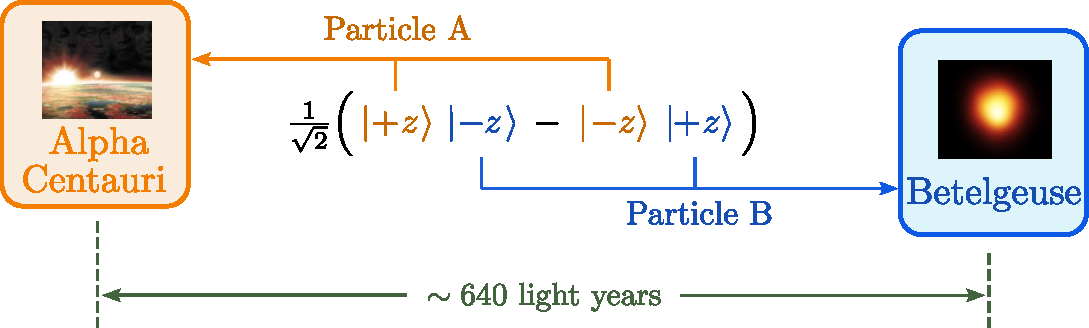
\includegraphics[width=0.75\textwidth]{epr}
\end{figure}

Once ready, an experimentalist at Alpha Centauri measures $\hat{S}_z$
on particle $A$, which induces an instantaneous collapse of the
two-particle state.  Immediately afterwards, another experimentalist
at Betelgeuse measures $\hat{S}_z$ on particle $B$, and obtains---with
100\% certainty---the opposite spin.  During the time interval between
these two measurements, no classical signal could have traveled
between the two star systems, not even at the speed of light.  Yet,
the state collapse induced by the measurement at Alpha Centauri has a
definite effect on the result of the measurement at Betelgeuse.

There are three noteworthy aspects of this phenomenon:

First, it dispels some intuitive-seeming but mistaken ``explanations''
of quantum state collapse.  For instance, it is sometimes explained
that if we want to measure a particle's position, we need to shine a
light beam on it, or disturb it in some way; due to this disturbance,
the particle's momentum becomes uncertain after the measurement.  The
EPR paradox shows that such stories don't capture the full weirdness
of quantum state collapse, since we can collapse the state of a
particle by doing a measurement on \textit{another} particle far away!

Second, the experimentalist has a certain amount of control over the
state collapse, due to the choice of what measurement to perform.  So
far, we have considered $S_z$ measurements performed on particle $A$.
But the experimentalist at Alpha Centauri can choose to measure the
spin of $A$ along another axis, say $S_x$.  In the basis of spin-up
and spin-down states, the operator $\hat{S}_x$ has matrix
representation
$$\hat{S}_x = \frac{\hbar}{2}\, \begin{pmatrix}0&1\\1&0\end{pmatrix}.$$
The eigenvalues and eigenvectors are
$$\begin{aligned}s_x = \;\;\frac{\hbar}{2},\; &\;\;\; |\!+\!x\rangle = \frac{1}{\sqrt{2}}\Big(|\!+\!z\rangle + |\!-\!z\rangle\Big) \\ s_x = -\frac{\hbar}{2}, &\;\;\; |\!-\!x\rangle = \frac{1}{\sqrt{2}}\Big(|\!+\!z\rangle - |\!-\!z\rangle\Big).\end{aligned}$$
Conversely, we can write the $\hat{S}_z$ eigenstates in the $\{|\!+\!x\rangle,|\!-\!x\rangle\}$ basis:
$$\begin{aligned}|\!+\!z\rangle &= \frac{1}{\sqrt{2}}\Big(|\!+\!x\rangle + |\!-\!x\rangle\Big) \\ |\!-\!z\rangle &= \frac{1}{\sqrt{2}}\Big(|\!+\!x\rangle - |\!-\!x\rangle\Big).\end{aligned}$$
This allows us to write the two-particle entangled state in the
$\hat{S}_x$ basis:
$$|\psi\rangle = \frac{1}{\sqrt{2}} \Big(|\!-\!x\rangle|\!+\!x\rangle \,-\, |\!+\!x\rangle|\!-\!x\rangle\Big).$$
The Alpha Centauri measurement still collapses the particles into
definite spin states with opposite spins---but now spin states of
${S}_x$ rather than ${S}_z$.

Third, the choice of measurement cannot be used for superluminal
communication.  The experimentalist at Alpha Centauri can choose
whether to (i) measure $S_z$ or (ii) measure $S_x$, and this choice
instantaneously affects the state of particle $B$.  If the Betelgeuse
experimentalist can find a way to distinguish between the cases (i)
and (ii), even statistically, this would serve as a method of
instantaneous communication, violating the theory of relativity!  Yet
this turns out to be impossible.  The key problem is that quantum
states themselves cannot be measured; only observables can be
measured.  Suppose the Alpha Centauri measurement is $\hat{S}_z$,
which collapses $B$ to either $|\!+\!z\rangle$ or $|\!-\!z\rangle$
(each with probability 0.5).  The Betelgeuse experimentalist must now
choose which measurement to perform.  If $S_z$ is measured, the
outcome is $+\hbar/2$ or $-\hbar/2$ with equal probabilities.  If
$S_x$ is measured, the probabilities are:
$$\begin{aligned}P(S_x = +\hbar/2) &= \frac{1}{2}\, \Big|\langle\!+x|\!+\!z\rangle\Big|^2 \;+\;\, \frac{1}{2}\, \Big|\langle\!+x|\!-\!z\rangle\Big|^2 = \frac{1}{2}\\P(S_x = -\hbar/2) &= \frac{1}{2}\, \Big|\langle\!-x|\!+\!z\rangle\Big|^2 \;+\;\, \frac{1}{2}\, \Big|\langle\!-x|\!-\!z\rangle\Big|^2 = \frac{1}{2},\end{aligned}$$
which has exactly the same distribution!  The analysis can be repeated
for any other choice of spin axis; we always find that the outcomes
occur with 50/50 probability.  Thus, the Betelgeuse measurement does
not yield any information about the choice of measurement axis at
Alpha Centauri.

Since quantum state collapse does not allow for superluminal
communication, it is consistent \textit{in practice} with the theory
of relativity.  However, state collapse is still \textbf{nonlocal}, in
the sense that certain unobservable ingredients of the theory (quantum
states) change faster than light can travel between two points.  For
this reason, EPR argued that quantum theory is
\textit{philosophically} inconsistent with relativity.

EPR suggested an alternative: maybe quantum mechanics is an
approximation of some deeper theory, whose details are currently
unknown, but which is deterministic and local.  Such a
``\textbf{hidden variables theory}'' may give the appearance of
quantum state collapse in the following way.  Suppose each particle
has a definite but ``hidden'' value of $S_z$, either $S_z = +\hbar/2$
or $S_z = -\hbar/2$; let us denote these as $[+]$ or $[-]$.  We can
hypothesize that the two-particle quantum state $|\psi\rangle$ is not
an actual description of reality; rather, it corresponds to a
\textit{statistical} distribution of ``hidden variable'' states,
denoted by $[+;-]$ (i.e., $S_z = +\hbar/2$ for particle $A$ and $S_z =
-\hbar/2$ for particle $B$), and $[-;+]$ (the other way around).

\begin{figure}[h]
  \centering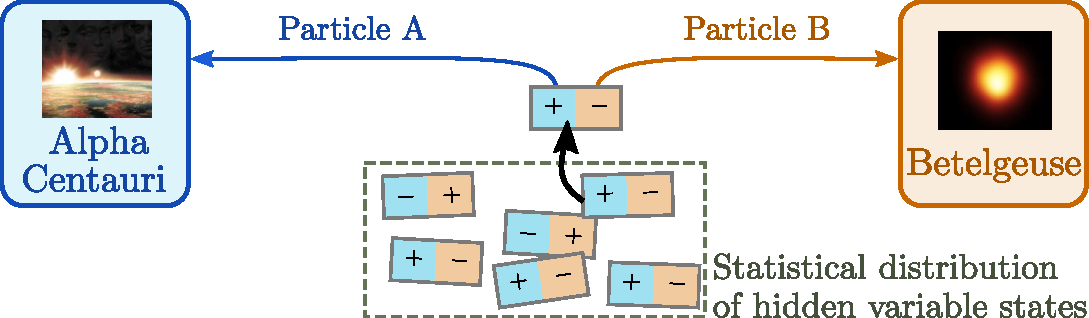
\includegraphics[width=0.75\textwidth]{hiddenvariables}
\end{figure}

When the Alpha Centauri experimentalist measures $S_z$, the value of
the hidden variable is revealed.  A result of $+z$ implies $[+;-]$,
whereas $-z$ implies $[-;+]$.  When the Betelgeuse experimentalist
subsequently measures $S_z$, the result obtained is the opposite of
the Alpha Centauri result.  But this happens simply because those were
the values all along---there is no instantaneous physical influence
traveling from Alpha Centauri to Betelguese.

Clearly, there are many missing details in this hidden variables
description.  In particular, such a theory would have to be consistent
with the huge list of successful predictions made by quantum theory.
Trying to come up with a suitable hidden variables theory seems
difficult, but with enough hard work, one might imagine that it is
doable.

\section{Bell's theorem}

In 1964, however, John S.~Bell published a
\hyperref[cite:bell]{bombshell paper} showing that the predictions of
quantum theory are \textit{inherently inconsistent} with hidden
variable theories.  The amazing thing about this result, known as
\textbf{Bell's theorem}, is that it requires no knowledge about the
details of the hidden variable theory, just that it is deterministic
and local.  Here, we present a simplified version of Bell's theorem,
based on \hyperref[cite:mermin]{Mermin (1981)}.

We again consider spin-1/2 particle pairs, with particle $A$ sent to
Alpha Centauri and particle $B$ sent to Betelgeuse.  At each location,
an experimentalist can measure the particle's spin along three
distinct choices of spin axis.  These spin observables are denoted by
$S_1$, $S_2$, and $S_3$.  We will not specify the actual directions of
these spin axes until later in the proof.  For now, just note that the
axes need not correspond to orthogonal spatial directions.

We now repeatedly prepare two-particle systems, and send the particles
to Alpha Centauri and Betelgeuse.  Each time, the prepared
two-particle state is
$$|\psi\rangle = \frac{1}{\sqrt{2}} \Big(|\!+\!z\rangle|\!-\!z\rangle \,-\, |\!-\!z\rangle|\!+\!z\rangle\Big).$$
During each round of the experiment, each experimentalist randomly
chooses one of the three spin axes $S_1$, $S_2$, or $S_3$, and
performs that spin measurement.  It doesn't matter which
experimentalist performs the measurement first; the experimentalists
can't influence each other, as there is not enough time for a
light-speed signal to travel between the two locations.  Many rounds
of the experiment are conducted; for each round, both
experimentalists' choices of spin axis are recorded, along with their
measurement results.

\begin{figure}[h]
  \centering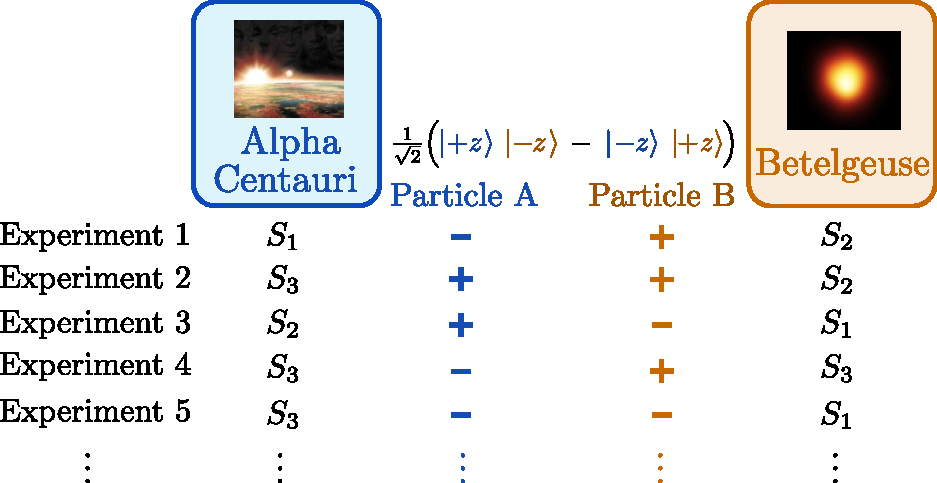
\includegraphics[width=0.67\textwidth]{bell}
\end{figure}

At the end, the experimental records are brought together and
examined.  We assume that the results are consistent with the
predictions of quantum theory.  Among other things, this means that
whenever the experimentalists happen to choose the same measurement
axis, they always find opposite spins.  (For example, this is the case
during ``Experiment 4'' in the above figure, where both
experimentalists happened to measure $S_3$.)

Can a hidden variables theory reproduce the results predicted by
quantum theory?  In a hidden variables theory, each particle must have
a definite value for each spin observable.  For example, particle $A$
might have $S_1 = +\hbar/2, \, S_2 = +\hbar/2, \, S_3 = -\hbar/2$.
Let us denote this by $[++-]$.  To be consistent with the predictions
of quantum theory, the hidden spin variables for the two particles
must have opposite values along each direction.  This means that there
are $8$ distinct possibilities, which we can denote as
$$\begin{aligned}{[}{+++};{---}], \;\;\; [{++-};{--+}], \;\;\; [{+-+};{-+-}], \;\;\; [{+--};{-++}],\\ [{-++};{+--}], \;\;\; [{-+-};{+-+}], \;\;\; [{--+};{++-}], \;\;\; [{---};{+++}].\end{aligned}$$
For instance, $[{++-};{--+}]$ indicates that for particle $A$, $S_1 =
S_2 = +\hbar/2$ and $S_3 = -\hbar/2$, while particle $B$ has the
opposite spin values, $S_1 = S_2 = -\hbar/2$ and $S_3 = +\hbar/2$.
So far, however, we don't know anything about the relative
probabilities of these 8 cases.

Let's now focus on the subset of experiments in which the two
experimentalists happened to choose \textit{different} spin axes
(e.g., Alpha Centauri chose $S_1$ and Betelgeuse chose $S_2$).  Within
this subset, what is the probability \textit{for the two measurement
  results to have opposite signs} (i.e., one $+$ and one $-$)?  To
answer this question, we first look at the following 6 cases:
$$\begin{aligned}{[}{++-};{--+}], \;\;\; [{+-+};{-+-}], \;\;\; [{+--};{-++}],\\ [{-++};{+--}], \;\;\; [{-+-};{+-+}], \;\;\; [{--+};{++-}].\end{aligned}$$
These are the cases which do not have all $+$ or all $-$ for each
particle.  Consider one of these, say ${[}{++-};{--+}]$.  The two
experimentalists picked their measurement axes at random each time,
and amongst the experiments where they picked different axes, there
are two ways for the measurement results to have opposite signs:
$(S_1,S_2)$ or $(S_2,S_1)$.  There are four ways to get the same sign:
$(S_1,S_3)$, $(S_2,S_3)$, $(S_3,S_1)$ and $(S_3, S_2)$.  Thus,
for this particular set of hidden variables, the probability for
measurement results with opposite signs is 1/3.  If we go through all
6 of the cases listed above, we find that in call cases, the
probability for opposite signs is 1/3.

Now look at the remaining 2 cases:
$${[}{+++};{---}], \;\;\; [{---};{+++}].$$
For these, the experimentalists always obtain results that have
opposite signs.  Combining this with the findings from the previous
paragraph, we obtain the following statement:

\textit{Given that the two experimentalists choose different spin
  axes, the probability that their results have opposite signs is $P
  \ge 1/3$.}

This is called \textbf{Bell's inequality}.  If we can arrange a
situation where quantum theory predicts a probability $P < 1/3$ (i.e.,
a violation of Bell's inequality), that would mean that quantum theory
is inherently inconsistent with local deterministic hidden variables.
This conclusion would hold regardless of the ``inner workings'' of the
hidden variables theory, because the above derivation made no
assumptions about any such details (such as the probabilities of the
hidden variable states).

To complete the proof, we must find a set $\{S_1, S_2, S_3\}$ such
that the predictions of quantum mechanics violate Bell's inequality.
One simple choice is to align $S_1$ with the $z$ axis, and align $S_2$
and $S_3$ along the $x$-$z$ plane at $120^\circ$ ($2\pi/3$ radians)
from $S_1$, as shown below:

\begin{figure}[h]
  \centering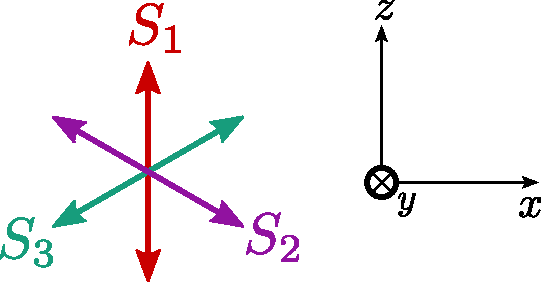
\includegraphics[width=0.35\textwidth]{bellaxes}
\end{figure}

The corresponding spin operators can be written in the eigenbasis of
$\hat{S}_z$:
$$\begin{aligned}\hat{S}_1 &= \frac{\hbar}{2} \, \sigma_3 \\ \hat{S}_2 &= \frac{\hbar}{2} \, \left[\cos(2\pi/3) \sigma_3 + \sin(2\pi/3)\sigma_1\right]  \\   \hat{S}_3 &= \frac{\hbar}{2} \, \left[\cos(2\pi/3) \sigma_3 - \sin(2\pi/3)\sigma_1\right].\end{aligned}$$

Suppose the Alpha Centauri experimentalist chooses $S_1$, and obtains
$+\hbar/2$.  Particle $A$ collapses to state $|\!+\!z\rangle$, and
particle $B$ collapses to state $|\!-\!z\rangle$.  The Betelgeuse
experimentalist is assumed to choose a different spin axis.  If the
choice is $S_2$, the expectation value is
$$\begin{aligned}\langle\, - z \, | \, S_2 \,|-\!z\,\rangle &= \frac{\hbar}{2} \Big[\cos(2\pi/3) \langle\,- z\,|\sigma_3| - \!z\,\rangle + \sin(2\pi/3)\langle\,- z\,|\sigma_1|-\!z\,\rangle\Big]\\ &= \frac{\hbar}{2} \cdot \frac{1}{2} \end{aligned}$$
If $P_+$ and $P_-$ respectively denote the probability of measuring
$+\hbar/2$ and $-\hbar/2$ in this measurement, the above equation
implies that $P_+ - P_- = + 1/2$.  Moreover, $P_+ + P_- = 1$ by
probability conservation.  It follows that the probability of
obtaining a negative value (the opposite sign from the Alpha Centauri
measurement) is $P_- = 1/4$.  All the other possible scenarios are
worked out in a similar way.

The result is that if the two experimentalists choose different
measurement axis, they obtain results of opposite signs with
probability $1/4$.  Therefore, Bell's inequality is violated.

Last of all, we must consult Nature itself.  Is it possible to
observe, in an actual experiment, probabilities that violate Bell's
inequality?  In the decades following Bell's 1964 paper, many
experiments were performed to answer this question.  These experiments
are all substantially more complicated than the simple two-particle
spin-$1/2$ model that we've studied, and they are subject to various
uncertainties and ``loopholes'' that are beyond the scope of our
discussion.  But in the end, the experimental consensus appears to be
a clear \textit{yes}: Nature really does behave according to quantum
mechanics, and in a manner that cannot be replicated by deterministic
local hidden variables!  A summary of the experimental evidence can be
found in \hyperref[cite:aspect]{Aspect (1999)}.

\section{Entanglement entropy}
\label{sec:entropy}

In previous sections, we said that a multi-particle system is
``entangled'' if the individual particles do not have definite quantum
states.  It would be nice to make this statement more precise, by
formulating an expression for the level of entanglement in any given
system.  In fact, physicists have come up with several ways of
quantifying entanglement; in this section, we will describe the most
commonly-used one, called \textbf{entanglement entropy}, which is
closely related to the concept of entropy in thermodynamics,
statistical mechanics, and information theory.

Consider a quantum system with a $d$-dimensional Hilbert space
$\mathscr{H}$.  Given an arbitrary state $|\psi\rangle \in
\mathscr{H}$, we can define an operator
$$\hat{\rho}(\psi) = |\psi\rangle\, \langle\psi|.$$
This is simply the projection operator associated with $|\psi\rangle$,
but in this context we call it a \textbf{density operator}.  In the
language of linear algebra, $\hat{\rho}(\psi)$ is formed by taking the
``matrix outer product'' of the vector $|\psi\rangle$ with its
Hermitian conjugate.  We use the notation $\hat{\rho}(\psi)$ to
emphasize that the density operator is dependent on the chosen state
$|\psi\rangle$.  Evidently, it is a Hermitian operator; one eigenvalue
is 1 (with eigenvector $|\psi\rangle$), and the other $d-1$
eigenvalues are all $0$ (with eigenvectors given by $d-1$ vectors
spanning the subspace orthogonal to $|\psi\rangle$).

The expectation values of the density operator have a special
significance.  Suppose the system is in state $|\psi\rangle$, and we
perform a measurement corresponding to the Hermitian operator
$\hat{Q}$, which has eigenvalues $\{q_1,q_2,\dots\}$ and eigenvectors
$\{|q_1\rangle,|q_2\rangle,\dots\}$.  The probability of measuring
$q_i$ is
$$P_i \;=\; |\langle q_i| \psi\rangle|^2 \;=\; \langle q_i |\psi\rangle \langle \psi|q_i\rangle \;=\; \langle q_i |\, \hat{\rho}(\psi)\, |q_i \rangle.$$
In other words, the expectation values of $\hat{\rho}(\psi)$
correspond to the probabilities for the outcomes of measurements
performed on $|\psi\rangle$.

Now suppose $\mathscr{H} = \mathscr{H}_A \otimes \mathscr{H}_B$, where
$\mathscr{H}_A$ and $\mathscr{H}_B$ are the Hilbert spaces of two
subsystems.  Starting from a density operator of the combined system,
$\hat{\rho}(\psi)$, we can define a \textbf{``reduced density
  operator''} for subsystem A:
$$\hat{\rho}_A(\psi) = \mathrm{Tr}_B \,\big[\,\hat{\rho}(\psi)\,\big].$$
Here, $\mathrm{Tr}_B[\cdots]$ refers to a \textbf{partial trace},
tracing over the Hilbert space of subsystem B.  What's left after
this partial trace is an operator acting solely on the Hilbert space
$\mathscr{H}_A$.

To understand the meaning of $\hat{\rho}_A(\psi)$, let us work in
an explicit basis.  Let $\{|\mu_1\rangle, |\mu_2\rangle,\cdots\}$ be a
basis for $\mathscr{H}_A$, and $\{|\nu_1\rangle,
|\nu_2\rangle,\cdots\}$ a basis for $\mathscr{H}_B$.  A given state of
the combined system can be written in the tensor product basis:
$$|\psi\rangle = \sum_{ij} \psi_{ij} \, |\mu_i\rangle  |\nu_j\rangle, \;\;\; \mathrm{where}\;\; \psi_{ij} \in \mathbb{C}.$$
The density operator of the combined system is
$$\hat{\rho}(\psi) = |\psi\rangle \langle\psi| = \sum_{ii'jj'} \Big( |\mu_i\rangle  |\nu_j\rangle\Big) \psi_{ij} \psi_{i'j'}^* \, \Big(\langle \mu_{i'}|  \langle \nu_{j'}|\Big).$$
The density operator for subsystem A is found by tracing over
the states of subsystem B:
$$\begin{aligned}\hat{\rho}_A(\psi) &= \sum_j \langle \nu_j | \hat{\rho}(\psi) | \nu_j \rangle \\ &= \sum_{ii'} |\mu_i\rangle \,\rho_{ii'}^A \, \langle \mu_{i'}| \;\;\;\mathrm{where} \;\; \rho_{ii'}^A \equiv \sum_j \psi_{ij} \psi_{i'j}^*.\end{aligned}$$
Note that $\hat{\rho}_A(\psi)$ is clearly Hermitian.

The density operator for subsystem A contains information about the
outcome probabilities for \textit{partial} measurements performed on
subsystem A.  Suppose the overall system is in state $|\psi\rangle$,
and we perform a measurement on subsystem A corresponding to a
Hermitian operator $\hat{\mu}$, which has eigenvectors
$\{|\mu_1\rangle,|\mu_2\rangle,\dots\}$.  Then the probability of
measuring $\mu_i$ is
$$\langle \mu_i | \hat{\rho}_A |\mu_i \rangle \,=\, \rho_{ii}^A \,=\, \sum_{j} |\psi_{ij}|^2.$$
(Note that this is consistent with the discussion of partial
measurements in Section~\ref{sec:partialmeasurements}.)  In other
words, the diagonal matrix elements of $\hat{\rho}_A$, in any basis,
specify the outcome probabilities for measurements corresponding to
that basis.  Conservation of probability implies that $\sum_i
\rho^A_{ii} = 1$, and hence that
$$\mathrm{Tr}\big[\rho_A\big] = 1.$$

In entangled systems, the density operator essentially takes over the
theoretical role of the quantum state.  In a single-particle or
unentangled system, we can define the quantum state and use it to
calculate the probabilities of various measurement outcomes.  However,
a system has no definite quantum state if it is entangled with other
systems.  Probabilities are instead calculated from the density
operator.

Given a density operator, we can define a quantity called the
\textbf{entanglement entropy}:
$$S_{\mathrm{ent.}} = - k_B \mathrm{Tr} \Big\{ \hat{\rho}\, \ln\!\big[\hat{\rho}\big]\Big\}.$$
Here, $S_{\mathrm{ent.}}$ refers to the entropy of the system or
subsystem described by density operator $\hat{\rho}$.  For instance,
if we use the density operator $\hat{\rho}_A$ in the above formula, we
get the entropy of subsystem A.  In this formula, $\ln[\cdots]$
denotes the logarithm of an operator, which is the inverse of the
exponential: $\ln(\hat{A}) = \hat{B} \Rightarrow \exp(\hat{B}) =
\hat{A}$.  The prefactor $k_B$ is Boltzmann's constant, and ensures
that $S_{\mathrm{ent.}}$ has the same units as thermodynamic entropy.

The definition of the entanglement entropy is based on an analogy with
the entropy concept from classical thermodynamics, statistical
mechanics and information theory.  In those classical contexts,
entropy is a quantitative measure of uncertainty (i.e, lack of
information) about a system's underlying microscopic state, or
``microstate''.  Suppose a system has $W$ possible microstates that
occur with probabilities $\{p_1, p_2, \dots, p_W\}$, satisfying
$\sum_i p_i = 1$.  Then we define the classical entropy
$$S_{\mathrm{cl.}} = - k_B \sum_{i=1}^W p_i \ln(p_i).$$
In a situation of complete certainty where the system is known to be
in a specific microstate $k$ ($p_i = \delta_{ik}$), the formula gives
$S_{\mathrm{cl.}} = 0$.  (Note that $x \ln(x)\rightarrow 0$ as
$x\rightarrow 0$).  In a situation of complete uncertainty where all
microstates are equally probable ($p_i = 1/W$), we get
$S_{\mathrm{cl.}} = k_B \ln W$, the entropy of a microcanonical
ensemble in statistical mechanics.  For any other distribution of
probabilities, it can be shown that the entropy lies between these two
extremes: $0 \le S_{\mathrm{cl.}}  \le k_B\ln W$.  For a review of the
properties of entropy, see Appendix C.

Entanglement entropy quantifies the uncertainty arising from an
entangled quantum subsystem's lack of a definite quantum state.  But
we need to be careful when extending classical notions of probability
to quantum systems.  As described above, when performing a measurement
whose possible outcomes are $\{\mu_1, \mu_2, \dots\}$, the probability
of getting $\mu_i$ is $p_i = \langle \mu_i | \hat{\rho}|\mu_i\rangle$.
However, it is problematic to directly substitute these probabilities
$\{p_i\}$ into the classical entropy formula, since they are
basis-dependent (i.e., the set of probabilities is dependent on the
choice of measurement).  The above definition for the entanglement
entropy, $S_{\mathrm{ent.}} = - k_B \mathrm{Tr} \big\{ \hat{\rho}\,
\ln[\hat{\rho}] \big\}$, bypasses this problem by using the trace,
which is basis-independent.  This also means that if we look
specifically at the eigenbasis for $\hat{\rho}$, denoted by
$\{|\mu'_i\rangle\}$, then
$$\begin{aligned}S_{\mathrm{ent.}} &= -k_B \sum_i \langle \mu'_i | \hat{\rho}\ln(\hat{\rho}) | \mu'_i\rangle  \\ &= - k_B \sum_i p_i' \ln(p_i') \;\;\;\mathrm{where}\;\;\hat{\rho}\,|\mu'_i\rangle = p_i' |\mu'_i\rangle\end{aligned}$$
In this basis, where the eigenvalues $p_i =
\langle\mu'_i|\hat{\rho}|\mu'_i\rangle$ are also the measurement
probabilities, the entanglement entropy is consistent with the
classical definition of entropy.

For an unentangled system, we can write $\hat{\rho} =
|\psi\rangle\langle\psi|$ for some state $|\psi\rangle$, so
$|\psi\rangle$ is itself an eigenstate of $\hat{\rho}$ with eigenvalue
1; hence, $S_{\mathrm{ent.}} = 0$.  Conversely, if we find that a
system has $S_{\mathrm{ent.}} \ne 0$, that implies that it is
entangled, and lacks a definite quantum state.

A system is \textbf{maximally entangled} if the density operator
eigenvalues (measurement probabilities) are all equal: i.e., $p_i' =
1/d$, where $d$ is the dimension of the Hilbert space.  In that case,
the entropy is $S_{\mathrm{ent.}} = k_B \ln(d)$.  In general, the
entanglement entropy lies between these two extremes, $0 \le
S_{\mathrm{ent.}} \le k_B\ln(d)$.

As an example, consider the following state of two spin-$1/2$ particles:
$$|\psi\rangle = \frac{1}{\sqrt{2}} \Big(|\!+\!z\rangle|\!-\!z\rangle \,-\, |\!-\!z\rangle|\!+\!z\rangle\Big).$$
The density operator for the two-particle system is
$$\hat{\rho}(\psi) = \frac{1}{2} \Big(|\!+\!z\rangle|\!-\!z\rangle \,-\, |\!-\!z\rangle|\!+\!z\rangle\Big) \Big(\langle+z|\langle-z| \,-\, \langle-z|\langle+z|\Big).$$
Tracing over the B subsystem gives the reduced density operator:
$$\hat{\rho}_A(\psi) = \frac{1}{2} \Big(|\!+\!z\rangle \langle+z| \,+\, |\!-\!z\rangle \langle-z|\Big).$$
This can be expressed as a matrix in the
$\{|\!+z\rangle,|\!-z\rangle\}$ basis:
$$\hat{\rho}_A(\psi) = \begin{pmatrix}\frac{1}{2} & 0 \\ 0 & \frac{1}{2}\end{pmatrix}.$$
Note that this satisfies $\mathrm{Tr}(\hat\rho_A) = 1$, as expected.
Next, we can use $\hat{\rho}_A$ to compute the entropy of subsystem A:
$$S_{\mathrm{ent.}}^A = -k_B\mathrm{Tr}\left\{\hat{\rho}_A\ln(\rho_A)\right\} = -k_B\mathrm{Tr}\begin{pmatrix}\frac{1}{2}\ln\left(\frac{1}{2}\right) & 0 \\ 0 & \frac{1}{2}\ln\left(\frac{1}{2}\right)\end{pmatrix} = k_B\ln(2).$$
This is the maximum possible entanglement entropy for a system with a
2D Hilbert space.  Hence, subsystems A and B are maximally entangled.

\section{The Many Worlds Interpretation}

We conclude this chapter by discussing a set of compelling but
controversial ideas arising from the phenomenon of quantum
entanglement: the \textbf{Many Worlds Interpretation} of quantum
theory.

So far, when describing the phenomenon of state collapse, we have
relied on the measurement postulate (see
Section~\ref{sec:partialmeasurements}), which is part of the
\textbf{Copenhagen Interpretation} of quantum mechanics.  This is how
quantum mechanics is typically taught, and how physicists think about
the theory when doing practical, everyday calculations.

However, the measurement postulate has two bad features:

First, it seems to stand apart from the other postulates of quantum
mechanics, in being the only place where randomness (or
``indeterminism'') creeps into quantum theory.  The other postulates
do not refer to probabilities.  In particular, the Schr\"odinger equation
$$i\hbar\frac{\partial}{\partial t}|\psi(t)\rangle = \hat{H}(t) |\psi(t)\rangle$$
is completely deterministic.  If you know $\hat{H}(t)$ and are given
the state $|\psi(t_0)\rangle$ at some time $t_0$, you can (in
principle) solve the Schr\"odinger equation to determine
$|\psi(t)\rangle$ for all $t$.  This time-evolution consists of a
smooth, non-random rotation of the state vector within its Hilbert
space.  A measurement process, however, has a completely different
character: it causes the state vector to jump discontinuously to a
randomly-selected value.  It is strange that quantum theory contains
two such different descriptions of state change.

Second, the measurement postulate is silent on what constitutes a
measurement.  Does measurement require a conscious observer?  Surely
not: as Einstein once exasperatedly asked, are we really expected to
believe that the Moon exists only when we look at it?  But then if a
given device interacts with a particle, what determines whether it
acts via the Schr\"odinger equation, or performs a measurement?

The Many Worlds Interpretation seeks to resolve these problems by
positing that \textit{the measurement postulate is \underline{not} a
  fundamental postulate of quantum mechanics}.  Rather, what we call
``measurement'', including state collapse and the apparent randomness
of measurement results, is an emergent phenomenon that can be derived
from the behavior of complex many-particle quantum systems obeying the
Schr\"odinger equation.  The key idea is that a measurement process
can be described by applying the Schr\"odinger equation to a quantum
system containing both the thing being measured \textit{and} the
measurement apparatus itself.

We can study this using a toy model formulated by
\hyperref[cite:albrecht]{Albrecht (1993)}.  Consider a spin-$1/2$
particle, and an apparatus designed to measure $S_z$.  Let
$\mathscr{H}_S$ be the spin-$1/2$ Hilbert space (which is 2D), and
$\mathscr{H}_A$ be the Hilbert space of the apparatus (which has
dimension $d$).  We will assume that $d$ is very large, as actual
experimental apparatuses are macroscopic objects containing $10^{23}$
or more atoms!  The Hilbert space of the combined system is
$$\mathscr{H} = \mathscr{H}_S \otimes \mathscr{H}_A,$$
and is $2d$-dimensional.  Let us suppose the system is prepared in an initial
state
$$|\psi(0)\rangle = \Big(a_+ |\!+z\rangle + a_- |\!-z\rangle\Big) \otimes |\Psi\rangle,$$
where $a_\pm\in\mathbb{C}$ are the quantum amplitudes for the particle
to be initially spin-up or spin-down, and $|\Psi\rangle \in
\mathscr{H}_A$ is the initial state of the apparatus.

The combined system now evolves via the Schr\"odinger equation.  We
aim to show that if the Hamiltonian has the form
$$\hat{H} = \hat{S}_z \otimes \hat{V},$$
where $\hat{S}_z$ is the operator corresponding to the observable
$S_z$, then time evolution has an effect equivalent to the measurement
of $S_z$.  To show this, it turns out that we do not need to make any
special choices for $\hat{V}$ or the initial apparatus state
$|\Psi\rangle$.  We only need $d \gg 2$, and for $|\Psi\rangle$ and
$\hat{V}$ to be both ``sufficiently complicated''.

In fact, we can choose $|\Psi\rangle$ to be a random state vector, and
choose random matrix components for the operator $\hat{V}$.  The
precise generation procedures will be elaborated on later.  Once we
decide on $|\Psi\rangle$ and $\hat{V}$, we can evolve the system by
solving the Sch\"odinger equation
$$|\psi(t)\rangle = U(t)|\psi(0)\rangle, \;\;\;\mathrm{where}\;\; \hat{U}(t) = \exp\left[-\frac{i}{\hbar}\hat{H}t\right].$$
Because the part of $\hat{H}$ acting on the $\mathscr{H}_S$ subspace
is $\hat{S}_z$, the result necessarily has the following form:
$$\begin{aligned}|\psi(t)\rangle &= \hat{U}(t)\Big(a_+ |\!+\!z\rangle + a_- |\!-\!z\rangle\Big) \otimes |\Psi\rangle \\ &= a_+ |\!+\!z\rangle \otimes |\Psi_+(t)\rangle \;+\; a_- |\!-\!z\rangle \otimes |\Psi_-(t)\rangle. \end{aligned}$$
Here, $|\Psi_+(t)\rangle$ and $|\Psi_-(t)\rangle$ are apparatus states
that are ``paired up'' with the $|\!+\!z\rangle$ and $|\!-\!z\rangle$
states of the spin-$1/2$ subsystem.  At $t=0$, both
$|\Psi_+(t)\rangle$ and $|\Psi_-(t)\rangle$ are equal to
$|\Psi\rangle$; for $t > 0$, they rotate into different parts of the
state space $\mathscr{H}_A$.  If the dimensionality of $\mathscr{H}_A$
is sufficiently large, and both $\hat{V}$ and $|\Psi\rangle$ are
sufficiently complicated, we can guess (and we will verify numerically) that
the two state vectors rotate into completely different parts of
the state space, so that
$$\langle\Psi_+(t) | \Psi_-(t)\rangle \approx 0 \;\;\;\textrm{for sufficiently large}\;\; t.$$
Once this is the case, the two terms in the above expression for
$|\psi(t)\rangle$ can be interpreted as two decoupled ``worlds''.  In
one world, the spin has a definite value $+\hbar/2$, and the apparatus
is in a state $|\Psi_+\rangle$ (which might describe, for instance, a
macroscopically-sized physical pointer that is pointing to a ``$S_z =
+\hbar/2$'' reading).  In the other world, the spin has a definite
value $-\hbar/2$, and the apparatus has a different state
$|\Psi_+\rangle$ (which might describe a physical pointer pointing to
a ``$S_z = -\hbar/2$'' reading).  Importantly, the $|\Psi_+\rangle$
and $|\Psi_-\rangle$ states are orthogonal, so they can be rigorously
distinguished from each other.  The two worlds are
``weighted'' by $|a_+|^2$ and $|a_-|^2$, which correspond to the
probabilities of the two possible measurement results.

The above description can be tested numerically.  Let us use an
arbitrary basis for the apparatus space $\mathscr{H}_A$; in that
basis, let the $d$ components of the initial apparatus state vector
$|\Psi\rangle$ be random complex numbers:
\begin{equation}
  |\Psi\rangle = \frac{1}{\sqrt{\mathcal{N}}}\, \begin{pmatrix}\Psi_0 \\ \Psi_1 \\ \vdots \\ \Psi_{d-1}
  \end{pmatrix}, \;\; \mathrm{where} \;\; \mathrm{Re}(\Psi_j), \mathrm{Im}(\Psi_j) \sim N(0,1).
\end{equation}
In other words, the real and imaginary parts of each complex number
$\Psi_j$ are independently drawn from the the standard normal
(Gaussian) distribution, denoted by $N(0,1)$.  The normalization
constant $\mathcal{N}$ is defined so that $\langle\Psi|\Psi\rangle =
1$.

Likewise, we generate the matrix elements of $\hat{V}$ according to
the following random scheme:
$$\begin{aligned}A_{ij} &\sim u_{ij} + i v_{ij}, \;\;\;\mathrm{where}\;\;u_{ij},v_{ij}\sim N(0,1)\\ \hat{V} &= \frac{1}{2\sqrt{d}} \left(\hat{A} + \hat{A}^\dagger\right).\end{aligned}$$
This scheme produces a $d\times d$ matrix with random components,
subject to the requirement that the overall matrix be Hermitian.  The
normalization factor $1/2\sqrt{d}$ is relatively unimportant; it
ensures that the eigenvalues of $\hat{V}$ lie in a fixed range,
$[-2,2]$, instead of scaling with $d$.  If you are interested in
learning more about the properties of such ``random matrices'', see
\hyperref[cite:edelman]{Edelman and Rao (2005)}.

The Schr\"odinger equation can now be solved numerically.  The results
are shown below:

\begin{figure}[h]
  \centering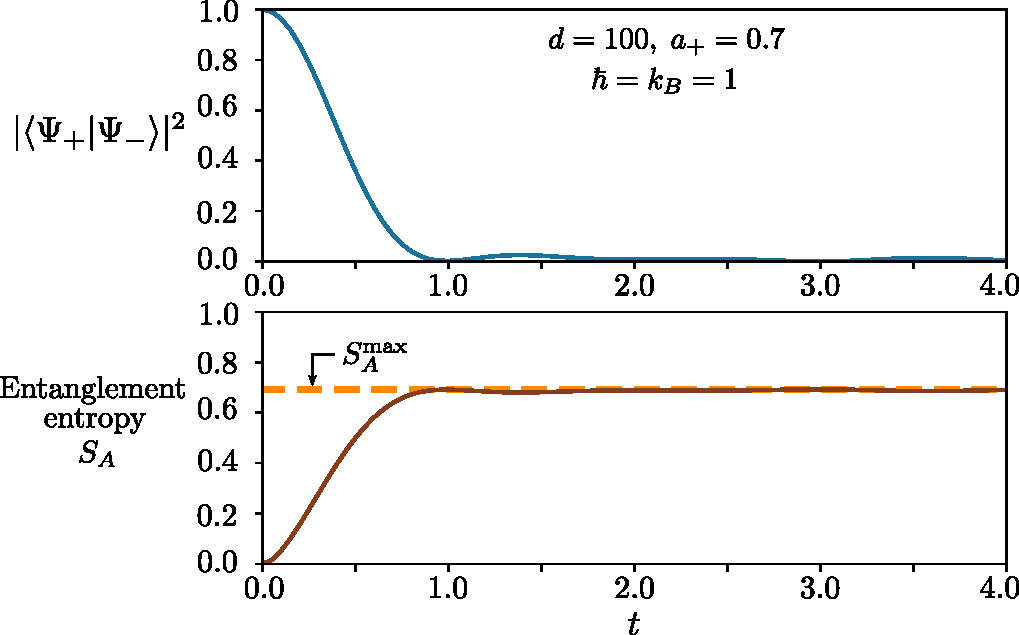
\includegraphics[width=0.7\textwidth]{decoherence}
\end{figure}

In the inital state, we let $a_+ = 0.7$, so $a_- = \sqrt{1-0.7^2} =
0.71414\dots$ The upper panel plots the overlap between the two
apparatus states, $|\langle\Psi_+|\Psi_-\rangle|^2$, versus $t$.  In
accordance with the preceding discussion, the overlap is unity at $t =
0$, but subsequently decreases to nearly zero.  For comparison, the
lower panel plots the entanglement entropy between the two subsystems,
$S_A = -k_B \mathrm{Tr}_A\left\{\hat{\rho}_A\ln\hat{\rho}_A\right\}$,
where $\hat{\rho}_A$ is the reduced density matrix obtained by tracing
over the spin subspace.  We find that $S_A = 0$ at $t=0$, due to the
fact that the spin and apparatus subsystems start out with definite
quantum states in $|\psi(0)\rangle$.  As the system evolves, the
subsystems become increasingly entangled, and $S_A$ increases up to
$$S_A^{\mathrm{max}}/k_B = - \Big( |a_+|^2 \ln|a_+|^2 + |a_-|^2\ln|a_-|^2 \Big) \approx 0.693$$
This value is indicated in the figure by a horizontal dashed line, and
corresponds to the result of the classical entropy formula for
probabilities $\{|a_+|^2,|a_-|^2\}$.  Moreover, we see that the
entropy reaches $S_A^{\mathrm{max}}$ at around the same time that
$|\langle\Psi_+|\Psi_-\rangle|^2$ reaches zero.  This demonstrates the
close relationship between ``measurement'' and ``entanglement''.

For details about the numerical linear algebra methods used to perform
the above calculation, refer to Appendix D.

The ``many worlds'' concept can be generalized from the above toy
model to the universe as a whole.  In the viewpoint of the Many Worlds
Interpretation of quantum mechanics, the entire universe can be
described by a mind-bogglingly complicated quantum state, evolving
deterministically according to the Schr\"odinger equation.  This
evolution involves repeated ``branchings'' of the universal quantum
state, which continuously produces more and more worlds.  The
classical world that we appear to inhabit is just one amidst a vast
multitude of worlds.  It is up to you to decide whether this
conception of reality seems reasonable.  It is essentially a matter of
preference, because the Copenhangen Interpretation and the Many Worlds
Interpretation have identical physical consequences (which is why they
are referred to as different ``interpretations'' of quantum mechanics,
rather than different theories).




\section*{Exercises}

\begin{enumerate}
\item \textcolor{red}{Prove that the inner product for tensor product basis states satisfies inner product axiom.}
\item \textcolor{red}{Calculate entropy for Bell states.}
\item \textcolor{red}{Explicit model for MWI state collapse.}
\end{enumerate}

\section*{Further Reading}

\begin{itemize}

\item Bransden \& Joachain, \S14.1---14.4, \S17.1--17.5

\item Sakurai, \S3.9

\item A.~Einstein, B.~Podolsky, and N.~Rosen,
  \textit{Can Quantum-Mechanical Description of Physical Reality Be
    Considered Complete?}, Physical Review \textbf{47}, 777 (1935).
  \label{cite:epr}

\item J.~S.~Bell, \textit{On the Einstein-Podolsky-Rosen paradox},
  Physics \textbf{1}, 195 (1964). \label{cite:bell}
  
\item N.~D.~Mermin, \textit{Bringing home the atomic world: Quantum
  mysteries for anybody}, American Journal of Physics \textbf{49}, 940
  (1981). \label{cite:mermin}

\item A.~Aspect, \textit{Bell's inequality test: more ideal than ever},
  Nature (News and Views) \textbf{398}, 189 (1999). \label{cite:aspect}

\item A.~Albrecht, \textit{Following a "collapsing" wave function},
  Physical Review D \textrm{48}, 3768 (1993).
\label{cite:albrecht}

\item A.~Edelman and N.~R.~Rao, \textit{Random matrix theory}, Acta
  Numerica \textbf{14}, 233 (2005).
\label{cite:edelman}
\end{itemize}

\end{document}


%% For decades after the discovery of quantum mechanics, the quantum
%% double-slit experiment was just a ``thought experiment'', meant to
%% illustrate the features of quantum mechanics that had been uncovered
%% by other, more complicated experiments.  Nowadays, the most convenient
%% way to do the experiment is with light, using single-photon sources
%% and single-photon detectors.  Quantum interference has also been
%% demonstrated experimentally using electrons, neutrons, and even
%% large-scale particles such as buckyballs.
